\documentclass[11pt]{article}
\usepackage[T1]{fontenc}
\usepackage{lmodern}
\usepackage{amsmath,amssymb,amsthm,mathtools}
\usepackage[margin=1.1in]{geometry}
\usepackage{microtype}
\usepackage{enumitem}
\usepackage{needspace}
\usepackage{tikz}
\usetikzlibrary{arrows.meta}
\usepackage[colorlinks=true,linkcolor=blue!45!black,citecolor=blue!45!black,urlcolor=blue!45!black]{hyperref}
\usepackage[nameinlink,noabbrev,capitalise]{cleveref}
\hypersetup{pdftitle={Integrability of split tangent bundles on rationally connected manifolds},pdfauthor={OpenAI}}

\newtheorem{theorem}{Theorem}[section]
\newtheorem{proposition}[theorem]{Proposition}
\newtheorem{lemma}[theorem]{Lemma}
\newtheorem{corollary}[theorem]{Corollary}
\theoremstyle{remark}
\newtheorem{remark}[theorem]{Remark}
\numberwithin{equation}{section}
\newcommand{\PP}{\mathbb P}
\newcommand{\CC}{\mathbb C}
\newcommand{\OO}{\mathcal O}
\newcommand{\BB}{\mathcal B}
\newcommand{\pr}{\operatorname{pr}}
\newcommand{\ev}{\operatorname{ev}}
\newcommand{\id}{\operatorname{id}}
\newcommand{\rk}{\operatorname{rank}}
\newcommand{\fm}{\mathfrak m}
\newcommand{\Span}{\operatorname{span}}
\newcommand{\wh}{\widehat}
\DeclareMathOperator{\Hom}{Hom}
\DeclareMathOperator{\length}{length}

\title{Integrability of split tangent bundles\\
on rationally connected manifolds}
\author{OpenAI}
\date{September 23, 2026}

\begin{document}
\maketitle

\begin{abstract}
We prove that both summands of every specified holomorphic splitting of the
tangent bundle of a smooth rationally connected projective complex manifold
into two positive-rank subbundles are integrable. This proves H\"oring's
conjecture on rationally connected projective manifolds. H\"oring's product
theorem then gives a product decomposition compatible with the specified
splitting.
\end{abstract}

\section{Introduction}

A product of complex manifolds has a tangent bundle split into the
pullbacks of the tangent bundles of its factors. A converse must keep
track of more than the abstract bundles. For a specified decomposition
\[
T_X=E_1\oplus E_2,
\]
the embeddings of \(E_1\) and \(E_2\) in \(T_X\) are part of the data,
and a compatible product must identify these subbundles with its factor
directions. A necessary local condition is \emph{integrability}:
the holomorphic local sections of each \(E_i\) must be closed under
the Lie bracket.

We prove that rational connectedness forces this local condition.
Here and below, ``two general points'' means all pairs in some nonempty
Zariski open subset of \(X\times X\). A smooth connected projective complex
manifold is rationally connected if two general points lie on the image
of a morphism \(\PP^1\to X\).

\begin{theorem}[Automatic integrability]\label[theorem]{thm:main}
Let \(X\) be a smooth connected projective complex manifold of dimension
at least two. Suppose that two general points of \(X\) lie on the image
of a morphism \(\PP^1\to X\). For every specified holomorphic decomposition
\[
T_X=E_1\oplus E_2
\]
into subbundles of positive rank, both \(E_1\) and \(E_2\) are integrable.
\end{theorem}

The theorem has no further rank or positivity hypothesis. It proves the
smooth rationally connected assertion formulated in
\cite[Conjecture~1.5]{Hor26}. H\"oring's earlier product theorem then
answers the global question for the same specified splitting.

\Needspace{7\baselineskip}
\begin{corollary}[Compatible product]\label[corollary]{cor:product}
Under the hypotheses of \cref{thm:main}, there are smooth projective
manifolds \(X_1,X_2\) and an isomorphism \(X\simeq X_1\times X_2\)
under which
\[
E_i=\pr_i^*T_{X_i}\qquad (i=1,2).
\]
\end{corollary}

\begin{proof}
H\"oring's \cite[Theorem~1.4]{Hor07} applies to a smooth connected
rationally connected projective complex manifold with a specified
splitting of its tangent bundle and at least one integrable summand.
By \cref{thm:main}, these hypotheses hold. His theorem gives an
isomorphism with a product that identifies the specified summands with
the factor tangent bundles. Each factor is smooth. It is projective
because its realization as a slice of the product is a closed complex
submanifold of \(X\), and a projective embedding of \(X\) restricts
to an embedding of that slice.
\end{proof}

\subsection*{Context and scope}

Beauville studied how a tangent-bundle splitting on a compact K\"ahler
manifold can lead to a product of its universal cover \cite{Bea00}.
An abstract product need not make a given summand integrable:
H\"oring's \cite[Example~2.14]{Hor07} gives a nonintegrable summand on
a product of an abelian surface with \(\PP^1\). Rational connectedness
rules out that example and supplies the abundance of rational curves
used in our proof.

Several earlier results establish compatible products under positivity
or rank assumptions. Campana and Peternell treated Fano manifolds with
a two-summand splitting when one summand has rank one or two, and hence
every two-summand splitting on a Fano manifold of dimension at most five
\cite[Theorems~3.5--3.6 and Corollary~3.7]{CP02}. H\"oring's
\cite[Theorem~1.4]{Hor07} showed that, for a rationally connected
projective manifold, integrability of one summand already gives a
compatible product. He then isolated the remaining question by
conjecturing that at least one summand is integrable
\cite[Conjecture~1.2]{Hor08}. His later low-rank result applies to a
uniruled projective manifold whose tangent bundle splits into summands
all of rank at most two, and proves that at least one of them is
integrable \cite[Lemma~4.21]{Hor08}.

The recent Fano-type theorem \cite[Theorem~1.1]{Hor26} establishes
integrability with algebraic leaves for split tangent sheaves on normal
\(\mathbb Q\)-factorial projective klt varieties of Fano type. In the
smooth Fano case it yields an actual compatible product
\cite[Corollary~1.3]{Hor26}. The present theorem removes this positivity
condition for smooth rationally connected manifolds. Smoothness matters:
\cite[Example~4.3]{Hor26} gives a singular rationally connected example
with a nonintegrable summand. Section~\ref{sec:consequences} applies the
smooth theorem to general fibers of the rationally connected quotient,
supplying the integrability premise in H\"oring's structure theorems
for uniruled compact K\"ahler manifolds.

\subsection*{Proof strategy}

The construction that drives the proof does not require rational
connectedness. Given any holomorphic map \(g:\PP^1\to X\) into a smooth
projective manifold with a split tangent bundle, we construct
\[
F:\PP^1\times\PP^1\longrightarrow X,\qquad F(s,s)=g(s),
\]
with the first factor direction tangent to \(E_1\) and the second
tangent to \(E_2\). We call \(F\) a \emph{tangent box}. The name records
these tangencies; the map may have critical points and need not give
local coordinates.

Write \(P_i:T_X\to E_i\subset T_X\) for the holomorphic projectors
defined by the splitting. The diagonal first carries a formal solution. In coordinates
\(u=s\), \(v=t-s\), the equation
\(\partial_v\widehat F=P_2(\widehat F)\partial_u\widehat F\)
recursively separates the derivative of \(g\) into its two summands.
The positive normal bundle of the diagonal then bounds the number of
global formal sections of a twisted line bundle. Comparing that bound
with pairs of polynomial sections forces the formal projective
coordinate ratios to be rational. A local cancellation makes these
ratios holomorphic near a diagonal patch. Finally, on a resolution of
the rational map, the two tangency identities force every exceptional
curve to be contracted. The resulting map is holomorphic on the entire
product. The section-count argument is given directly for holomorphic
formal series; the algebraic formal-function literature provides
broader context \cite{HM68,Bad96}.

The splitting also provides the projected-bracket partial connection
\(\nabla^i_\xi e=P_i[\xi,e]\) on \(E_i\) in directions of the
complementary summand. On a tangent box it gives transport along the
fibers of \(\pr_i\), which vary the complementary factor, and hence
\[
F^*E_i\simeq\pr_i^*(g^*E_i),
\]
normalized to be the identity on the diagonal. Thus, on a factor curve,
the corresponding summand retains the bundle \(g^*E_i\), while the
complementary summand is trivial.

Rational connectedness enters only in the last step. A two-point family
of rational curves supplies sections of \(g^*E_i\) that vanish at one
marked point and span the summand at another. Applying the bracket tensor
\(\bigwedge^2E_i\to E_j\) to two such sections on a factor curve gives
a section of a trivial bundle on \(\PP^1\). It is constant and vanishes
at the first mark, so it vanishes at the second. The spanning property
then kills the bracket tensor on an open set of \(X\), and hence
everywhere. The use of rational curves to annihilate this tensor has a
direct antecedent in \cite[Section~2.B and Lemma~3.18]{Hor07}; the tangent
box supplies the trivial complementary target in arbitrary rank.

\subsection*{Organization}

\Cref{sec:boxes} constructs tangent boxes through the formal Cauchy
problem, rational reconstruction, and removal of indeterminacy.
\Cref{sec:transport} establishes the bundle identifications, and
\cref{sec:vanishing} proves \cref{thm:main}. The rational-quotient
consequence follows in \cref{sec:consequences}. Appendix~\ref{app:surface}
proves the required point-blowup resolution for a surface, and
Appendix~\ref{app:variation} derives the two-point family directly from
rational connectedness.

\section{Tangent boxes}\label{sec:boxes}

Throughout this section, \(X\) is a smooth projective complex manifold
with a fixed splitting \(T_X=E_1\oplus E_2\).
Let \(P_i:T_X\to E_i\subset T_X\) be the corresponding holomorphic
projectors. Put
\[
C=\PP^1,\qquad S=C\times C,\qquad
\Delta=\{(s,s):s\in C\},
\]
and write \(T^{(i)}=\pr_i^*T_C\subset T_S\).

\begin{proposition}[Tangent box]\label[proposition]{prop:box}
Every holomorphic map \(g:C\to X\) admits a holomorphic map \(F:S\to X\)
such that
\begin{equation}\label{eq:box}
F|_\Delta=g,\qquad
dF(T^{(1)})\subset F^*E_1,\qquad
dF(T^{(2)})\subset F^*E_2.
\end{equation}
Neither summand is assumed integrable.
\end{proposition}

The proof has three stages. The projectors first determine a formal
map along \(\Delta\). A count of formal sections then produces a
rational map with that expansion near part of the diagonal. Finally,
the two tangency conditions force every exceptional curve in a
resolution to be contracted, so the rational map is holomorphic on
all of \(S\).

\subsection{The formal Cauchy problem}

We specify the analytic formal neighborhood in which the first stage
takes place. Let \(\mathcal I\subset\OO_S\) be the analytic ideal
sheaf of \(\Delta\), and let \(\iota:\Delta\hookrightarrow S\) be
the inclusion. On the topological space \(\Delta\), set
\[
\wh{\OO}_{S,\Delta}
 =\varprojlim_{n\ge0}\iota^{-1}(\OO_S/\mathcal I^{n+1}),
\qquad
\wh{\mathcal I}=\ker(\wh{\OO}_{S,\Delta}\longrightarrow\OO_\Delta).
\]
Thus the analytic completion is the ringed space
\(\wh S_\Delta=(\Delta,\wh{\OO}_{S,\Delta})\). On a diagonal
coordinate disk with coordinates \(u=s\), \(v=t-s\), its structure
sheaf is \(\OO_\Delta[[v]]\), and \(\wh{\mathcal I}=(v)\).
The coefficients are holomorphic along the disk; convergence in the
normal variable \(v\) is not required.

A formal holomorphic map \(\wh G:\wh S_\Delta\to Y\) to a complex
manifold \(Y\) consists of a holomorphic diagonal map
\(g_0:\Delta\to Y\) and a morphism of sheaves of \(\CC\)-algebras
\[
\wh G^\#:g_0^{-1}\OO_Y\longrightarrow\wh{\OO}_{S,\Delta}
\]
reducing to \(g_0^\#\) modulo \(\wh{\mathcal I}\). We require this
map to be given locally by holomorphic Taylor substitution, as follows.
On a source disk with the above \(\OO_\Delta[[v]]\) description,
view functions of \(u\) as constant series in \(v\).
In target coordinates \(z=(z^1,\ldots,z^q)\), put
\(f=(\wh G^\#z^1,\ldots,\wh G^\#z^q)\) and
\(\eta=f-z\circ g_0\in\wh{\mathcal I}^{\oplus q}\). For a
holomorphic function \(h\) on the target chart, substitution at order
\(n\) is
\[
\wh G^\#h\bmod\wh{\mathcal I}^{n+1}
 =\sum_{|\alpha|\le n}
   \frac{(\partial^\alpha h)(z\circ g_0)}{\alpha!}\,
   \eta^\alpha\bmod\wh{\mathcal I}^{n+1}.
\]
Every monomial in \(\eta\) of total degree \(n+1\) is zero at this
order, so the sum is finite.
These substitutions are compatible as \(n\) varies and preserve
products and holomorphic coordinate changes. Consequently, one can
specify a formal map by coordinate series with the stated constant
terms, provided that on overlaps they agree by these substitutions.
The same rule then determines the pullback of every holomorphic
function, not only of the coordinate functions.

A source holomorphic vector field \(D\) satisfies
\(D(\mathcal I^{k+1})\subset\mathcal I^k\) for \(k\ge0\), and
hence acts as a continuous derivation on the completion. Locally,
\(\partial_u\) differentiates the coefficients of a series and
\(\partial_v\) differentiates its powers of \(v\). A derivation
can lower the normal order, so it need not define a derivation on any one fixed-order
thickening. Formal differential identities below are equalities in
the completion. In target coordinates they are equalities of vectors
of formal series; the formal chain rule makes them independent of the
target coordinates.

\begin{lemma}\label[lemma]{lem:formal}
There is a unique formal holomorphic map \(\wh F\) along \(\Delta\)
with diagonal value \(g\) and the two tangency properties in
\eqref{eq:box}, interpreted formally.
\end{lemma}

\begin{proof}
Use the same coordinate on a source chart in each factor, denoting
the two coordinates by \(s,t\). Set
\[
u=s,\qquad v=t-s.
\]
After restricting the diagonal disk so that \(g\) takes values in
one target coordinate chart, impose
\begin{equation}\label{eq:cauchy}
\wh F(u,0)=g(u),\qquad
\partial_v\wh F=P_2(\wh F)\partial_u\wh F.
\end{equation}
Here the entries of the holomorphic matrix \(P_2\) are substituted
by the Taylor rule above. That rule preserves \(P_2^2=P_2\) and
\(P_1+P_2=\id\).

Because \(\partial_u=\partial_s+\partial_t\) and
\(\partial_v=\partial_t\), \eqref{eq:cauchy} is equivalent to
\[
P_1(\wh F)\partial_t\wh F=0,\qquad
P_2(\wh F)\partial_s\wh F=0.
\]
Indeed, the equation puts \(\partial_v\wh F\) in the image of
\(P_2(\wh F)\), while applying \(P_2(\wh F)\) to
\(\partial_u\wh F-\partial_v\wh F\) gives zero. Conversely,
these two statements recover \eqref{eq:cauchy}. They are exactly
the two formal tangency conditions.

Write \(\wh F=\sum_{k\ge0}f_k(u)v^k\), with \(f_0=g\) in the
chosen coordinates. At order zero, \eqref{eq:cauchy} gives
\[
f_1=P_2(g)g'.
\]
Thus along the diagonal the second-factor derivative is
\(P_2(g)g'\), and the first-factor derivative is its complement
\(g'-f_1=P_1(g)g'\). The higher coefficients extend this forced
first-order decomposition. The coefficient of \(v^k\) on the
right side of \eqref{eq:cauchy} involves only
\(f_0,\ldots,f_k\) and their \(u\)-derivatives. It determines
\((k+1)f_{k+1}\), so induction gives a unique solution whose
coefficients are holomorphic on the diagonal disk.

We verify that these local solutions define a formal map globally.
Under a target-coordinate change \(z'=\psi(z)\), Taylor substitution
gives \(\wh F'=\psi(\wh F)\), and the formal chain rule gives
\(D\wh F'=d\psi(\wh F)D\wh F\). The matrix of \(P_2\) changes
by the corresponding conjugation, so \eqref{eq:cauchy} is preserved.
For a source change \(s'=h(s)\), \(t'=h(t)\), one has
\[
u'=h(u),\qquad v'=h(u+v)-h(u).
\]
The new normal parameter is \(v\) times a unit, so this substitution
identifies the two completions. With
\[
a=\frac1{h'(u)},\qquad b=\frac1{h'(u+v)},
\]
the continuous source derivations transform as
\[
\partial_{v'}=b\partial_v,\qquad
\partial_{u'}=a\partial_u+(b-a)\partial_v.
\]
Since \(P_2(\wh F)\partial_v\wh F=\partial_v\wh F\), these
formulas imply
\[
P_2(\wh F)\partial_{u'}\wh F
 =b\partial_v\wh F=\partial_{v'}\wh F.
\]
The initial value also transforms to the same diagonal map. Local
uniqueness therefore identifies the coordinate series on every
overlap. Their Taylor substitution maps agree as well, since those
maps are determined by the coordinate series. This proves both
global existence and uniqueness.
\end{proof}

\subsection{Rational reconstruction along the diagonal}

We next recover an ordinary rational map from the formal one. The
positive normal bundle of \(\Delta\) bounds the number of formal
sections after twisting; comparison with pairs of polynomial sections
then forces each formal coordinate ratio to be rational. The
classical study of algebraic formal rational functions provides
background for this mechanism; see Hironaka--Matsumura \cite{HM68}
and B\u{a}descu \cite{Bad96}. The proof below works
directly in the analytic completion just defined, including the
passage to an ordinary holomorphic map near the diagonal.

We use the notation
\(\OO_S(m,m)=\pr_1^*\OO_C(m)\otimes\pr_2^*\OO_C(m)\).

\Needspace{7\baselineskip}
\begin{lemma}\label[lemma]{lem:rational}
Let \(Y\subset\PP^N\) be a closed complex submanifold and let
\(\wh G\) be a formal holomorphic map from the formal neighborhood
of \(\Delta\subset S\) to \(Y\).
There is a rational map \(R:S\dashrightarrow\PP^N\) that is
holomorphic on a neighborhood of a nonempty open subset of
\(\Delta\), where its formal expansion agrees with \(\wh G\).
On that neighborhood it takes values in \(Y\).
\end{lemma}

\begin{proof}
Write \(g_0=\wh G|_\Delta\). We first construct the formal pullback
of \(\OO_{\PP^N}(1)\). Choose a cover of \(g_0(\Delta)\) by
affine projective charts \(U_a\) with holomorphic frames \(e_a\)
of this line bundle, and write \(e_b=t_{ab}e_a\) on overlaps.
Restricting \(t_{ab}\) to \(Y\) and applying \(\wh G^\#\) gives
formal functions \(\wh t_{ab}\) on
\(g_0^{-1}(U_a\cap U_b)\). Their constant terms are
\(t_{ab}\circ g_0\), which are nowhere zero. Thus each
\(\wh t_{ab}\) is a unit in the completion. The substitutions
preserve the transition cocycle identities, so the relations
\(\wh e_b=\wh t_{ab}\wh e_a\) glue free rank-one modules into a
locally free \(\wh{\OO}_{S,\Delta}\)-module \(L\).

If the homogeneous coordinate section \(x_\nu\) is
\(c_{\nu,a}e_a\) on \(U_a\), evaluate \(c_{\nu,a}|_Y\) by the
same substitution. The resulting local sections
\(\wh G^\#(c_{\nu,a}|_Y)\wh e_a\) agree on overlaps, giving global
sections \(S_0,\ldots,S_N\) of this very module \(L\).
Its reduction \(L_0=L/\wh{\mathcal I}L\) is the ordinary
holomorphic line bundle \(g_0^*\OO_{\PP^N}(1)\) on \(\Delta\simeq C\).
The reductions of the coordinate sections have no common zero, so
after reordering, \(S_0|_\Delta\) is not identically zero. Its zero
divisor has some degree \(d\ge0\) and identifies
\[
L_0\simeq\OO_C(d).
\]
For example, a degree-\(d\) homogeneous polynomial with the same
zero divisor gives this identification directly.

For a fixed \(m\ge0\), let \(\wh{\OO}_S(m,m)\) denote the restriction of
the ordinary line bundle to the completion, and put
\[
\mathcal M_m=L\otimes_{\wh{\OO}_{S,\Delta}}\wh{\OO}_S(m,m),
\qquad V=H^0(\Delta,\mathcal M_m),
\]
\[
V_k=H^0(\Delta,\wh{\mathcal I}^{\,k}\mathcal M_m)\subset V
\quad(k\ge0).
\]
Thus \(V_0=V\), and \(V_k\) consists precisely of global formal
sections vanishing to normal order at least \(k\). Passing a section
to its class modulo \(\wh{\mathcal I}^{k+1}\mathcal M_m\) has
kernel \(V_{k+1}\). It gives the leading-coefficient injection
\begin{equation}\label{eq:graded}
V_k/V_{k+1}\hookrightarrow
H^0\bigl(C,\OO_C(d+2m-2k)\bigr).
\end{equation}
Indeed, the leading-coefficient sheaf is
\[
\frac{\wh{\mathcal I}^{\,k}\mathcal M_m}
     {\wh{\mathcal I}^{\,k+1}\mathcal M_m}
\simeq L_0\otimes\OO_S(m,m)|_\Delta
             \otimes\iota^{-1}(\mathcal I^k/\mathcal I^{k+1}).
\]
Only the constant terms of the frame transitions act on this
quotient. Since \(\Delta\) has bidegree \((1,1)\), its conormal
bundle \(\mathcal I/\mathcal I^2\) is \(\OO_C(-2)\); the displayed
sheaf is therefore \(\OO_C(d+2m-2k)\), as asserted.

This filtration is separated. In a formal frame a section is a
series in \(v\), so membership in every \(V_k\) makes every
coefficient zero. For all sufficiently large \(k\), the space on
the right side of \eqref{eq:graded} is zero. Hence, for some \(K\),
\(V_k=V_{k+1}\) for every \(k\ge K\), and
\(V_K=\bigcap_{k\ge K}V_k=0\) by separatedness. The finite remaining
filtration gives
\begin{equation}\label{eq:sectionbound}
\dim_\CC V
\le\sum_{k\ge0}\max\{d+2m-2k+1,0\}
=m^2+O(m+1).
\end{equation}
Here \(d\) is fixed. More explicitly, the sum is
\((m+q+1)^2\) for \(d=2q\) and
\((m+q+1)(m+q+2)\) for \(d=2q+1\).

Restrict ordinary polynomial sections of \(\OO_S(m,m)\) to the
completion. For each \(\nu=1,\ldots,N\), consider
\[
H^0(S,\OO_S(m,m))^{\oplus2}\longrightarrow V,\qquad
(A,B)\longmapsto AS_0+BS_\nu.
\]
Its source has dimension \(2(m+1)^2\). Choose \(m\) large enough
that this exceeds the bound in \eqref{eq:sectionbound}, and choose
a nonzero kernel pair \((A_\nu,B_\nu)\) for each \(\nu\).

Fix a connected diagonal coordinate disk \(D\) on which
\(S_0|_\Delta\) is nowhere zero, contained in one product affine
chart. The section \(S_0\) is then a formal frame for \(L\) along
\(D\), and \(S_\nu/S_0\) is the substituted affine coordinate
\(x_\nu/x_0\). Necessarily \(B_\nu\ne0\): otherwise \(A_\nu S_0=0\)
would say that the ordinary section \(A_\nu\) has zero formal
expansion along \(D\). Its convergent local Taylor series would
make it zero on a neighborhood of \(D\), and the identity principle
on connected \(S\) would give \(A_\nu=0\), a contradiction.
The ratios
\[
q_\nu=-A_\nu/B_\nu\in\CC(S)
\]
therefore define a rational map \(R=[1:q_1:\cdots:q_N]\).

It remains to show that these ratios are holomorphic simultaneously
near one point of \(D\). Use \(u=s\), \(v=t-s\) and an ordinary
frame for \(\OO_S(m,m)\) on the chosen product chart, and represent
\(A_\nu,B_\nu\) by holomorphic functions \(a_\nu(u,v)\),
\(b_\nu(u,v)\). Write their normal Taylor coefficients on \(D\)
as \(a_{\nu,k}(u)\), \(b_{\nu,k}(u)\). For each \(\nu\), the
generic normal order
\[
r_\nu=\min\{k\ge0:b_{\nu,k}\text{ is not identically zero on }D\}
\]
is finite. Otherwise Taylor uniqueness near \(D\), followed by
the identity principle on \(S\), would make the nonzero ordinary
section \(B_\nu\) vanish identically. Each leading coefficient
\(b_{\nu,r_\nu}\) is a nonzero holomorphic function on the connected
disk \(D\). Its zeros are discrete, so a single point \(p\in D\)
can be chosen where all the finitely many leading coefficients are
nonzero.

In the formal frame \(S_0\), the kernel relations become
\[
a_\nu+b_\nu(S_\nu/S_0)=0
\quad\text{in }\OO_D[[v]].
\]
By the definition of \(r_\nu\), all coefficients of \(b_\nu\)
below that order vanish on \(D\); the relation makes the same true
of \(a_\nu\). Since \(a_\nu\) and \(b_\nu\) are ordinary
holomorphic functions, this formal vanishing implies actual
holomorphic divisibility near \(p\):
\[
a_\nu=v^{r_\nu}\widetilde a_\nu,\qquad
b_\nu=v^{r_\nu}\widetilde b_\nu,
\qquad
\widetilde b_\nu(p)=b_{\nu,r_\nu}(p)\ne0.
\]
Indeed, their convergent Taylor expansions in \(v\) have the first
\(r_\nu\) coefficients zero. Shrink to one neighborhood of \(p\)
where every \(\widetilde b_\nu\) is a holomorphic unit.
Multiplication by \(v\) is injective on formal series, so the same
power can be canceled in each formal relation. It follows that
\[
q_\nu=-\widetilde a_\nu/\widetilde b_\nu
\]
is holomorphic there and has formal expansion \(S_\nu/S_0\).
Thus \(R\) is holomorphic on this common neighborhood. Its affine
coordinate series agree with those of the composition of \(\wh G\)
with \(Y\hookrightarrow\PP^N\). The Taylor substitution rule then
makes these formal maps agree on every holomorphic function on the
projective target chart.

Finally, \(R(p)=g_0(p)\), so shrink the source neighborhood until
its image lies in a target chart with holomorphic defining equations
for \(Y\).
Their compositions with \(R\) have zero normal Taylor series,
because their substitutions by \(\wh G\) are zero. The convergent
Taylor series of these ordinary holomorphic functions make them
vanish on a neighborhood of \(p\). There \(R\) takes values in
\(Y\). In local submanifold coordinates, every holomorphic function
on \(Y\) extends to the ambient chart. The ambient formal equality
therefore also gives equality of the formal maps to \(Y\), as required.
\end{proof}

\begin{remark}\label[remark]{rem:g3}
The normal-bundle calculation in \eqref{eq:sectionbound} is the
rationality mechanism in the proof. The related algebraic language
uses the \(G_3\) property: the restriction map from rational
functions on the ambient variety to formal rational functions along
the subvariety is an isomorphism. The proof above does not invoke a
\(G_3\) theorem. Its section count and cancellation work directly
with the given holomorphic formal series, without an
analytic-to-algebraic comparison.
\end{remark}

\subsection{Complementary tangency removes indeterminacy}

Rational reconstruction has produced a map only away from its base
points. We next use the specified splitting to show that no base point
can remain: each exceptional curve would have to map tangentially to
both complementary summands, forcing its image to be a point.

\begin{lemma}\label[lemma]{lem:removal}
Let \(R:S\dashrightarrow X\) be a rational map such that, on its
domain of definition,
\[
dR(T^{(1)})\subset R^*E_1,\qquad
dR(T^{(2)})\subset R^*E_2.
\]
Then \(R\) extends to a holomorphic map \(S\to X\).
\end{lemma}

\begin{proof}
Choose a projective embedding \(X\subset\PP^N\).
By \cref{lem:surface}, there are a finite set \(B\subset S\), a
composition of point blowups \(\mu:S'\to S\) over \(B\), and a
holomorphic map \(F':S'\to\PP^N\) extending \(R\circ\mu\).
Since \(X\) is closed and \(F'\) maps a dense open set into \(X\),
the entire image lies in \(X\).

We show that \(F'\) is constant on each exceptional component.
Let \(H\) be such a component, lying over \(p\in B\), and let
\(s,t\) be coordinates on the two source factors near \(p\).
On the inverse image of this coordinate neighborhood,
\(P_i dF'\) is a holomorphic one-form with values in \(F'^*T_X\).
The tangency assumptions imply the identities
\begin{equation}\label{eq:wedges}
(P_1dF')\wedge d(s\circ\mu)=0,\qquad
(P_2dF')\wedge d(t\circ\mu)=0.
\end{equation}
The two wedge expressions are sections of the locally free sheaf
\(\Omega^2_{S'}\otimes F'^*T_X\). The identities first hold off
the exceptional curves, where \(\mu\) is an isomorphism, and then
hold everywhere by holomorphicity.

Both coordinate functions \(s\circ\mu-s(p)\) and
\(t\circ\mu-t(p)\) vanish along \(H\), since \(\mu(H)=\{p\}\).
Their generic orders along \(H\) are positive and finite. Indeed,
in a normal coordinate along a connected disk of \(H\), the first
normal Taylor coefficient that is not identically zero gives that
order. If no such coefficient existed, the pullback would vanish on
an open neighborhood meeting the dense locus where \(\mu\) is an
isomorphism, which is impossible for a coordinate function. Denote
the two respective orders by \(\alpha,\beta\). This reasoning
applies also to components created by later blowups.
At a general point of \(H\), avoiding intersections with other
components and zeros of the two leading coefficients, choose a
local equation \(r=0\). We can then write
\[
s\circ\mu-s(p)=r^\alpha h,\qquad
t\circ\mu-t(p)=r^\beta\widetilde h
\]
with holomorphic units \(h,\widetilde h\).

The first identity in \eqref{eq:wedges} is therefore
\[
r^{\alpha-1}(P_1dF')\wedge(\alpha h\,dr+r\,dh)=0.
\]
The holomorphic local ring of the smooth surface is a domain, so
multiplication by \(r^{\alpha-1}\) is injective on the locally free
module of bundle-valued two-forms. It can therefore be canceled.
At \(r=0\),
evaluate the resulting ambient two-form on a vector \(w\) tangent
to \(H\) and a vector \(n\) with \(dr(n)=1\). The result is
\(\alpha h\,P_1dF'(w)=0\), hence \(P_1dF'(w)=0\).
Canceling \(r^{\beta-1}\) in the second identity gives
\(P_2dF'(w)=0\) in the same way. Since \(P_1+P_2=\id\), the
derivative of \(F'|_H\) vanishes on a dense open subset of \(H\),
and hence everywhere. Since \(H\) is connected, \(F'|_H\) is constant.

The fibers of \(\mu\) away from \(B\) are points. Each nontrivial
fiber over \(B\) is a connected union of exceptional components:
the first blowup creates an exceptional line, and every later blowup
over that point replaces its center by a new line meeting the strict
transforms of the components through it, as in \cref{lem:surface}.
The constants on intersecting components agree,
so \(F'\) is constant on every fiber.

The map \(\mu\) is a continuous surjection from a compact space to
a Hausdorff space. It is therefore a quotient map, and \(F'\)
descends to a continuous map \(F:S\to X\), holomorphic off \(B\).
Near each point of \(B\), continuity places the image in a single
target coordinate chart. The coordinate functions are continuous
and holomorphic away from the isolated point. One-variable
removability on coordinate lines makes them separately
holomorphic, and the iterated Cauchy formula makes them
holomorphic. Hence \(F\) is holomorphic everywhere.
\end{proof}

\begin{proof}[Proof of \cref{prop:box}]
Apply \cref{lem:formal} and then \cref{lem:rational} to a projective
embedding of \(X\). The resulting rational map is holomorphic near
a nonempty diagonal patch and has formal expansion \(\wh F\) there.
Continuous differentiation and Taylor substitution identify the
expansions of \(P_1(R)\partial_tR\) and \(P_2(R)\partial_sR\)
with the zero formal tangency expressions of \(\wh F\). These are
ordinary holomorphic expressions, so Taylor uniqueness makes them
zero on a neighborhood of that patch. Let \(B\) be the finite base set from
\cref{lem:surface}. The complement \(S\setminus B\) is connected;
one can perturb any path in the connected real four-manifold \(S\)
inside coordinate balls to avoid the finitely many points.
The inverse image of \(X\) under the holomorphic map
\(R:S\setminus B\to\PP^N\) is an analytic subset containing a
nonempty open set, so it is all of \(S\setminus B\). The two
tangency conditions are then vanishing identities for holomorphic
bundle morphisms on this connected complement, and continue there
by the identity principle.

Now \cref{lem:removal} gives a holomorphic extension \(F:S\to X\).
Tangency extends by holomorphicity. The maps \(F|_\Delta\) and
\(g\) agree on the original nonempty diagonal patch, so they
agree on all of \(\Delta\).
\end{proof}

\section{Bundles on a tangent box}\label{sec:transport}

A tangent box separates the two bundles as well as the two tangent
directions. We show that each pulled-back summand comes from its
corresponding factor. Transport from the diagonal gives a natural
normalization of this identification at the point where the bracket
will be tested.

For \(i\ne j\), the splitting defines a projected-bracket partial
connection on \(E_i\) in directions of \(E_j\):
\begin{equation}\label{eq:partial}
\nabla^i_\xi e=P_i[\xi,e],
\end{equation}
where \(\xi\) and \(e\) are local holomorphic sections of \(E_j\)
and \(E_i\), respectively.

\Needspace{7\baselineskip}
\begin{proposition}\label[proposition]{prop:transport}
Let \(F:S\to X\) be a tangent box of \(g:C\to X\). Transport along
the fibers of \(\pr_i\) gives holomorphic bundle isomorphisms
\begin{equation}\label{eq:transport}
\Theta_i:\pr_i^*(g^*E_i)\xrightarrow{\ \sim\ }F^*E_i,
\qquad i=1,2,
\end{equation}
whose restrictions to the diagonal are the identity.
\end{proposition}

\begin{proof}
The bracket rules and \(P_i\xi=0\) give
\[
\nabla^i_{f\xi}e=f\nabla^i_\xi e,\qquad
\nabla^i_\xi(fe)=\xi(f)e+f\nabla^i_\xi e.
\]
Thus \eqref{eq:partial} is tensorial in its \(E_j\) direction and obeys
the connection Leibniz rule in its \(E_i\) argument. These two rules
use no bracket of two \(E_j\) sections and require no integrability
of either summand.

Fix \(i\) and let \(j\ne i\). The tangency of \(F\) sends the vertical
line bundle \(\ker(d\pr_i)=T^{(j)}\) into \(F^*E_j\). The partial
connection therefore pulls back to a holomorphic connection on
\(F^*E_i\) relative to \(\pr_i\). We spell out this construction because
\(F\) may have critical points. Take local frames \(e_\lambda\) of
\(E_i\) and \(\xi_\gamma\) of \(E_j\), and write
\[
\nabla^i_{\xi_\gamma}e_\lambda
 =\sum_\nu\Gamma_{\gamma\lambda}^{\nu}e_\nu,\qquad
dF(V)=\sum_\gamma h_\gamma F^*\xi_\gamma
\]
for a local holomorphic vertical vector field \(V\) on \(S\). Define
\[
D_V\!\left(\sum_\lambda f_\lambda F^*e_\lambda\right)
=\sum_\lambda V(f_\lambda)F^*e_\lambda
 +\sum_{\gamma,\lambda,\nu}
 f_\lambda h_\gamma
 (\Gamma_{\gamma\lambda}^{\nu}\circ F)F^*e_\nu.
\]
The two connection rules and the chain rule
\(V(A\circ F)=dA(dF(V))\) give the usual connection transformation
under a change of the \(E_i\) frame; tensoriality in the first argument
handles a change of the \(E_j\) frame. Hence these formulas agree on
overlapping product neighborhoods. They define a holomorphic relative
connection
\[
D:\mathcal O(F^*E_i)\longrightarrow
\mathcal O(F^*E_i\otimes\Omega^1_{S/C}),
\]
where the relative differential is for \(\pr_i:S\to C\). At a point where
\(dF(V)=0\), all \(h_\gamma\) vanish there and the formula still applies;
no inverse of \(dF\) is used.

The restriction of \(D\) to any fiber \(C=\PP^1\) is a holomorphic
connection. Its curvature is a holomorphic two-form on that curve and
therefore vanishes. Horizontal sections satisfy an everywhere nonsingular
holomorphic linear ordinary differential equation. Local existence and
uniqueness give continuation along every path, with reverse transport as
its inverse. Flatness and simple connectedness of \(\PP^1\) make this
transport path-independent. Starting at the fiber's diagonal point
therefore identifies its bundle with the corresponding fiber of
\(g^*E_i\).

These identifications depend holomorphically on both variables. Fix a
base point and a path in its fiber from the diagonal to a desired endpoint.
Cover the path by a finite chain of coordinate disks and bundle frames,
and shrink the base neighborhood so that the same chain applies to nearby
fibers. In each disk the coefficient matrix of the horizontal equation
is holomorphic in the base and fiber coordinates. Picard iteration
converges normally on smaller disks by the exponential-series estimate,
so its solution matrix is holomorphic in the base and the start and end
coordinates. Composing these local transports and frame changes gives a
holomorphic identification near the chosen point of \(S\). Path
independence makes the local identifications agree globally. Transport
at the starting diagonal point is the identity, giving \(\Theta_i\)
and its stated normalization.
\end{proof}

\section{Vanishing of the bracket tensors}\label{sec:vanishing}

We now test the bracket obstruction on sections supplied by deformations
of a rational curve. The tangent box makes the complementary target
bundle trivial along the curve where the test is performed. This use of
rational curves to force bracket vanishing has an antecedent in
\cite[Section~2.B and Lemma~3.18]{Hor07}.

Return to the hypotheses of \cref{thm:main}. For \(i\ne j\), define
\[
\BB_i:\bigwedge\nolimits^2E_i\longrightarrow E_j,\qquad
\BB_i(e,e')=P_j[e,e'].
\]
The extra terms in the bracket of scalar multiples lie in \(E_i\),
so \(P_j\) kills them. Thus \(\BB_i\) is a holomorphic bundle
morphism, and \(E_i\) is integrable exactly when \(\BB_i=0\).

The following consequence of rational connectedness gives the needed
sections. Its direct parameter-space proof is in
Appendix~\ref{app:variation}.

\begin{lemma}\label[lemma]{lem:variation}
Fix distinct \(a,b\in C\). There are a nonempty complex manifold
\(T\) and a holomorphic map \(G:C\times T\to X\) such that
\[
(\ev_a,\ev_b):T\longrightarrow X\times X,\qquad
\tau\longmapsto (G(a,\tau),G(b,\tau))
\]
is a submersion.
In particular, for \(g=G(\,\cdot\,,\tau)\), the global sections
of \(g^*E_i\) vanishing at \(a\) have values spanning \(E_i\) at
\(g(b)\).
\end{lemma}

\begin{proof}[Proof of \cref{thm:main}]
Choose the family in \cref{lem:variation}. For each member \(g\), take a
tangent box \(F:S\to X\) from \cref{prop:box}; the boxes need not be
chosen holomorphically as the member varies. For \(j\ne i\), consider
\[
L_i=\{(s_1,s_2)\in S:s_j=b\}.
\]
The free coordinate identifies \(L_i\) with \(C\). As shown in
\cref{fig:box}, its marked endpoint \((b,b)\) lies on the diagonal.
By \cref{prop:transport}, \(\Theta_i\) identifies
\(F^*E_i|_{L_i}\) with \(g^*E_i\), while \(\Theta_j\) identifies
\(F^*E_j|_{L_i}\) with the trivial bundle having fiber \(E_{j,g(b)}\).

Let \(u,v\) be any two global sections of \(g^*E_i\) vanishing at
\(a\). Restricting the transport maps to \(L_i\), the tensor value
\[
\sigma_{u,v}
=\Theta_j^{-1}\!\left((F^*\BB_i)(\Theta_i u\wedge\Theta_i v)\right)
\in H^0\bigl(C,\OO_C\otimes E_{j,g(b)}\bigr)
\]
is a holomorphic section of a trivial bundle on \(\PP^1\), hence is
constant. It vanishes at the point with free coordinate \(a\), so it
also vanishes at the point with free coordinate \(b\). At this latter
point, \(F(b,b)=g(b)\) and both transport maps are the identity.
Consequently
\[
\BB_i(g(b))\bigl(u(b)\wedge v(b)\bigr)=0.
\]
By \cref{lem:variation}, the values \(u(b)\) of sections vanishing at
\(a\) span \(E_{i,g(b)}\). Their pairwise wedges span its exterior
square, and therefore \(\BB_i(g(b))=0\).

This applies to both \(i\) and every member of the family. The map
\(\ev_b\) is a submersion, being the composition of the two-point
submersion with the second projection. Its image is a nonempty open
subset of \(X\), on which both bracket tensors vanish. The identity
principle for holomorphic bundle morphisms on connected \(X\) makes
them vanish everywhere. This is precisely integrability of both
specified summands.
\end{proof}

\begin{figure}[ht]
\centering
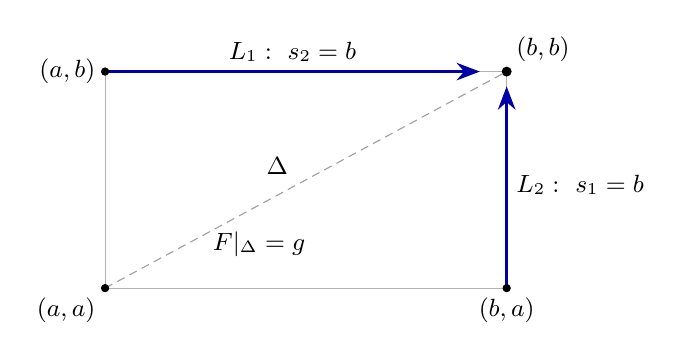
\begin{tikzpicture}[x=1.7cm,y=1.25cm,>=Stealth,
 every node/.style={font=\small}]
 \draw[gray!60] (0,0) rectangle (3,2.2);
 \draw[densely dashed,gray!75] (0,0)--(3,2.2)
 node[pos=.48,above left,text=black] {\(\Delta\)};
 \draw[very thick,blue!65!black,->] (0,2.2)--(2.8,2.2);
 \draw[very thick,blue!65!black,->] (3,0)--(3,2.05);
 \fill (0,0) circle (1.5pt);
 \fill (0,2.2) circle (1.5pt);
 \fill (3,0) circle (1.5pt);
 \fill (3,2.2) circle (1.8pt);
 \node[below left] at (0,0) {\((a,a)\)};
 \node[left] at (0,2.2) {\((a,b)\)};
 \node[below] at (3,0) {\((b,a)\)};
 \node[above right] at (3,2.2) {\((b,b)\)};
 \node[above] at (1.4,2.2) {\(L_1:\ s_2=b\)};
 \node[right] at (3,1.05) {\(L_2:\ s_1=b\)};
 \node at (1.15,.45) {\(F|_\Delta=g\)};
\end{tikzpicture}
\caption{The two factor curves used to test the bracket tensors,
drawn schematically in \(C\times C\).
On \(L_i\simeq\PP^1\), the input bundle is \(g^*E_i\) and the
complementary target bundle is trivial. Sections that vanish at
the marked off-diagonal point force their tensor values to
vanish at \((b,b)\), which maps to \(g(b)\).}
\label{fig:box}
\end{figure}



\section{Consequences for the rationally connected quotient}
\label{sec:consequences}

The main theorem also applies to the general fiber of the rationally
connected quotient of a uniruled compact K\"ahler manifold. That fiber
is a smooth projective manifold even when the ambient manifold is not
projective. Its tangent splitting is therefore integrable, which supplies
the premise in H\"oring's structure theorems \cite{Hor08}.

\begin{corollary}\label[corollary]{cor:rational-quotient}
Let \(X\) be a connected uniruled compact K\"ahler manifold with a
holomorphic splitting \(T_X=V_1\oplus V_2\). Let \(Z\) be a general
fiber of its rationally connected quotient and set
\(W_i=T_Z\cap V_i|_Z\).
For each \(i=1,2\), there is an almost-holomorphic fibration
\(\phi_i:X\dashrightarrow Y_i\) whose general fiber \(F_i\) is rationally
connected and, for compatible choices \(F_i\subset Z\), satisfies
\[
T_{F_i}=W_i|_{F_i}\subset V_i|_{F_i}.
\]
If \(W_i=0\), one may take \(\phi_i=\id_X\), with point fibers.

If \(\rk V_1=2\), exactly one of the following holds:
\begin{enumerate}[label=(\roman*)]
\item \(W_1=V_1|_Z\), and \(X\) admits an analytic fiber bundle
\(X\to Y\) with rationally connected general fiber and \(T_{X/Y}=V_1\).
\item \(W_1\) is a line bundle, and there is an equidimensional
holomorphic map \(X\to Y\) whose general fiber \(F\) is a rational curve
with \(T_F\subset V_1|_F\).
\item \(W_1=0\), equivalently \(T_Z\subset V_2|_Z\).
\end{enumerate}
\end{corollary}

\begin{proof}
Use the published version of \cite{Hor08}; its definition of an
almost-holomorphic fibration includes the identity case. Choose \(Z\)
over a regular value in the fibration locus of the quotient supplied by
\cite[Definition~2.9 and Theorem~2.10]{Hor08}. Then \(Z\) is an actual
smooth connected compact submanifold of \(X\). It inherits a K\"ahler
form and is rationally connected. Campana's theorem, recalled in the
remark after \cite[Definition~2.8]{Hor08}, makes \(Z\) projective.

By \cite[Proposition~3.16]{Hor08}, the ambient complementary projections
preserve \(T_Z\). Their restrictions are complementary holomorphic
idempotents. An idempotent has locally constant rank, so on connected
\(Z\) their images are the holomorphic subbundles \(W_i\), and
\[
T_Z=W_1\oplus W_2.
\]
If both ranks are positive, then \(\dim Z\ge2\), and \cref{thm:main}
makes both \(W_i\) integrable. Otherwise they are \(0\) and \(T_Z\),
which are integrable as well.

This is the general-fiber integrability hypothesis of
\cite[Theorem~1.3]{Hor08}, which gives the fibrations \(\phi_i\) and the
stated tangent identities. Its proof includes the identity when
\(W_i=0\). If \(\rk V_1=2\), \cite[Theorem~1.4]{Hor08} gives the three
conclusions according as \(\rk W_1\) is \(2\), \(1\), or \(0\).
These ranks are mutually exclusive and exhaustive, proving the stated
trichotomy.
\end{proof}

\appendix

\section{Elementary elimination of surface base points}
\label{app:surface}

Elimination of indeterminacy by point blowups is a classical part of
the birational theory of smooth surfaces; see \cite{Bea96}. The next
lemma supplies exactly the resolution statement used in
\cref{lem:removal}. We include the argument to make explicit the finite
termination of the point-blowup process, using the colength of the local
base ideal as the decreasing positive integer.

\begin{lemma}\label[lemma]{lem:surface}
A rational map \(R:\PP^1\times\PP^1\dashrightarrow\PP^N\) is
holomorphic outside a finite set \(B\). A finite sequence of
point blowups over \(B\) gives a smooth projective surface
\(\mu:S'\to\PP^1\times\PP^1\) on which \(R\circ\mu\) extends
holomorphically.
The fibers of \(\mu\) are connected; its exceptional components
are smooth curves.
\end{lemma}

\begin{proof}
Clear denominators to represent \(R\) by a tuple of
bihomogeneous polynomials of the same bidegree, and remove
all common factors. The factors can be taken bihomogeneous:
the highest and lowest degrees in each variable group are
additive in products.

In any product affine chart, the dehomogenized tuple
\(h_0(x,y),\ldots,h_N(x,y)\) has no common nonconstant factor.
Otherwise bihomogenizing such a factor would give a common
factor of the original tuple. In \(\CC(x)[y]\), the tuple
therefore has gcd one. A univariate B\'ezout identity, with
denominators cleared, puts a nonzero polynomial in \(x\)
in the ideal \((h_0,\ldots,h_N)\). Interchanging the variables
gives a nonzero polynomial in \(y\). The common zero set
in the affine chart is finite. At each common zero, the ideal
in centered formal coordinates contains powers of both
coordinates and consequently has finite colength.
There are four product affine charts, so the global base set
\(B\) is finite.

If \(B=\varnothing\), the map is already holomorphic, and
\(S'=S\), \(\mu=\id_S\) give the conclusion. Assume from now on
that \(B\ne\varnothing\).

It remains to resolve such a base point. Let
\[
D=\CC[[x,y]],\qquad \fm=(x,y),
\]
and let \(I\subset D\) be the ideal of a representing holomorphic
tuple \(f_0,\ldots,f_N\) at the point. Assume \(I\) is proper
and has finite colength, and let
\(k=\min_\nu\operatorname{ord}(f_\nu)\ge1\).
Blow up the point. In a chart \((x,z)\mapsto(x,xz)\), divide
the pulled-back tuple by \(x^k\); the divided functions are
holomorphic. The other chart gives the same map, since the
two tuples differ by a unit on their overlap.

On the exceptional projective line, the remaining base points
are common zeros of the degree-\(k\) initial forms.
At least one such form is nonzero, so there are finitely many.
Fix one. A linear change of the old coordinates lets us place
it at \((x,z)=(0,0)\) in the displayed chart. Let
\[
J=(x^{-k}f_\nu(x,xz))_\nu\subset\CC[[x,z]],
\qquad D'=\CC[[x,z]]/J.
\]
A power \(x^\ell\) belongs to \(I\); applying the substitution
and division gives \(x^{\ell-k}\in J\).
Thus the class of \(x\) in \(D'\) is nilpotent.
Modulo \(x\), a nonzero degree-\(k\) initial form gives a
nonzero polynomial in \(z\) of degree at most \(k\). Its
germ at the new base point is \(z^q\) times a unit, with
\(1\le q\le k\). Therefore \(D'/(x)\) is spanned by
\(1,z,\ldots,z^{k-1}\).
Successively lifting modulo the powers of the nilpotent \(x\)
shows that \(D'\) is spanned by finitely many classes
\(x^az^b\), with \(0\le b<k\).

There is a well-defined \(\CC\)-linear map
\begin{equation}\label{eq:transform}
\fm^k/I\longrightarrow D',\qquad
h\longmapsto x^{-k}h(x,xz).
\end{equation}
Indeed a monomial \(x^ay^b\) of total degree at least \(k\)
maps to \(x^{a+b-k}z^b\). All exponents are nonnegative, and
the resulting orders tend to infinity with the original
orders, so the operation is defined on arbitrary formal series.
If \(h=\sum_\nu q_\nu f_\nu\) lies in \(I\), its transform is
\(\sum_\nu q_\nu(x,xz)x^{-k}f_\nu(x,xz)\in J\).
This proves descent to the quotient; no multiplicativity is
needed.

Each spanning monomial \(x^az^b\), \(b<k\), is the image of
\(x^{a+k-b}y^b\in\fm^k\), so \eqref{eq:transform} is surjective.
It follows that
\begin{equation}\label{eq:lengthdrop}
\dim_\CC D'
\le \dim_\CC(\fm^k/I)
=\dim_\CC(D/I)-\frac{k(k+1)}2
<\dim_\CC(D/I).
\end{equation}
In particular, the new base ideals have finite colength, and
that positive integer decreases strictly along every surviving
branch of the blowup process.

There are finitely many initial base points and finitely many
children at each step. The maximum initial colength bounds
the length of every branch by \eqref{eq:lengthdrop}. Thus the
entire tree is finite, and finitely many point blowups remove
all base points. The local divided tuples define the desired
holomorphic map.

Finally, a point blowup is proper, has a projective line over
its center, and is an isomorphism elsewhere.
The strict transform of a smooth curve remains smooth, and
a new exceptional line meets the strict transforms of the
components through the center. Induction gives smooth
exceptional components and connected fibers of the composite.
\end{proof}

\section{Two-point evaluation from rational connectedness}
\label{app:variation}

We prove \cref{lem:variation} using only polynomial presentations
of maps from \(\PP^1\), analytic subsets, and the holomorphic
constant-rank theorem. This isolates the precise two-point variation
property used in the proof. For broader background on rationally
connected varieties, see \cite{KMM92,Kol99}.

We first record an elementary covering observation.
If \(A\) is a proper closed analytic subset of a connected
second-countable complex manifold \(M\), then \(A\) is covered
by countably many complex submanifolds of dimension smaller
than \(\dim M\). The covering submanifolds need not be contained
in \(A\).
To see this, choose a countable cover of \(A\) by sufficiently small connected
coordinate neighborhoods on which \(A\) is defined by holomorphic
functions. In each neighborhood choose a non-identically-zero defining
function \(f\). Such a function exists because a proper analytic subset
has empty interior.
At a zero of \(f\), let \(r\ge1\) be its finite order.
Some derivative of order \(r-1\) vanishes there and has
nonzero differential. Thus that point belongs to the regular
zero locus of one of the partial derivatives of \(f\).
There are countably many such derivatives and charts.
Their regular zero loci, with connected components separated,
give the asserted covering.

\begin{proof}[Proof of \cref{lem:variation}]
Embed \(X\) in \(\PP^N\). Every holomorphic map
\(C=\PP^1\to\PP^N\) is represented by a tuple of homogeneous
polynomials of a degree \(d\ge0\), with no common zero.
Indeed its pullback of \(\OO_{\PP^N}(1)\) is \(\OO_C(d)\),
and its homogeneous coordinate sections supply such a tuple.
For fixed \(d\), these tuples form an open subset \(M_d\)
of a finite-dimensional vector space. Openness follows
from compactness of \(C\).
There is a universal holomorphic evaluation map
\(C\times M_d\to\PP^N\).

We cover the tuples whose maps land in \(X\) by countably
many manifold families all of whose maps land in \(X\).
Start with the connected components of \(M_d\).
For a current connected submanifold \(M\), either every tuple
maps \(C\) into \(X\), in which case accept this family, or
there are \(\tau\in M\) and \(c\in C\) with
\(G(c,\tau)\notin X\). In the latter case
\[
\{\eta\in M:G(c,\eta)\in X\}
\]
is a proper closed analytic subset of \(M\), and contains
every desired tuple in \(M\).
Use the covering observation to replace it by countably
many lower-dimensional submanifolds, and repeat the same
test on each. All desired tuples survive. Extra points
introduced by the covering cause no problem: each new
manifold is tested anew. Dimension strictly decreases
whenever a family is not accepted. In dimension zero the
test accepts precisely the desired points. Finite depth
and countable branching give countably many accepted
families covering all the desired tuples.
On an accepted family the universal evaluation factors
holomorphically through the embedded submanifold \(X\).

Perform this construction for every \(d\). The resulting
countably many two-point evaluation maps to \(X\times X\)
have images containing general pairs: a rational curve
through two distinct points can be reparametrized to take
those values at the fixed distinct points \(a,b\).
By the convention in the introduction, these images contain a nonempty
Zariski open subset of \(X\times X\). It is also open in the usual
topology and has positive measure in smooth local coordinates.

Suppose, for a contradiction, that every one of these
evaluation maps has complex rank everywhere less than
\(2\dim X\). The image of each is then measure zero.
Here is a direct verification of that fact for a holomorphic
map \(\phi:M\to X\times X\) with the stated rank bound.
We may take \(M\) connected. On the open set of maximum
rank, the constant-rank theorem places the image locally
in a submanifold of smaller dimension than \(X\times X\).
Countably many local charts give a measure-zero image.
If the maximum rank is zero, this already treats all of \(M\).
Otherwise its complement is a proper closed analytic
subset. Cover that subset by countably many
lower-dimensional submanifolds and apply induction on
\(\dim M\). The strict rank bound persists on every such
restriction, including the extra points of a covering
submanifold. The zero-dimensional case is immediate.
This proves the asserted measure-zero property.

A countable union of measure-zero images cannot contain
that open subset. Some family therefore has a point where
two-point evaluation is submersive. Restrict its parameter
space to the nonempty open set where the differential is
surjective; call the resulting manifold \(T\).

Finally, a parameter tangent vector differentiates the
holomorphic family to a global section of \(g^*T_X\).
Surjectivity of the two-point evaluation differential
provides, for every \(w\in T_{g(b)}X\), such a section with
values \(0,w\) at \(a,b\). Projecting with \(P_i\) gives the
last assertion of \cref{lem:variation}.
\end{proof}


\begin{thebibliography}{10}
\raggedright

\bibitem{Bad96}
L.~B\u{a}descu,
\emph{Algebraic Barth--Lefschetz theorems},
Nagoya Math. J. \textbf{142} (1996), 17--38.
\href{https://doi.org/10.1017/S0027763000005626}
{doi:10.1017/S0027763000005626}.

\bibitem{Bea96}
A.~Beauville,
\emph{Complex algebraic surfaces}, second edition,
London Mathematical Society Student Texts \textbf{34},
Cambridge University Press, Cambridge, 1996.
\href{https://doi.org/10.1017/CBO9780511623936}
{doi:10.1017/CBO9780511623936}.

\bibitem{Bea00}
A.~Beauville,
\emph{Complex manifolds with split tangent bundle},
in \emph{Complex Analysis and Algebraic Geometry},
de Gruyter, Berlin, 2000, pp.~61--70.
\href{https://arxiv.org/abs/math/9809033v2}
{arXiv:math/9809033v2}.

\bibitem{CP02}
F.~Campana and T.~Peternell,
\emph{Projective manifolds with splitting tangent bundle, I},
Math. Z. \textbf{241} (2002), no.~3, 613--637.
\href{https://doi.org/10.1007/s00209-002-0435-5}
{doi:10.1007/s00209-002-0435-5}.
Theorem numbering follows
\href{https://arxiv.org/abs/math/0101198v1}
{arXiv:math/0101198v1}.

\bibitem{HM68}
H.~Hironaka and H.~Matsumura,
\emph{Formal functions and formal embeddings},
J. Math. Soc. Japan \textbf{20} (1968), nos.~1--2, 52--82.
\href{https://doi.org/10.2969/jmsj/02010052}
{doi:10.2969/jmsj/02010052}.

\bibitem{Hor07}
A.~H\"oring,
\emph{Uniruled varieties with split tangent bundle},
\href{https://arxiv.org/abs/math/0505327v3}
{arXiv:math/0505327v3}.
Published in Math. Z. \textbf{256} (2007), 465--479.
The title and theorem numbering used here follow the preprint.

\bibitem{Hor08}
A.~H\"oring,
\emph{The structure of uniruled manifolds with split tangent bundle},
Osaka J. Math. \textbf{45} (2008), no.~4, 1067--1084.
\href{https://www.i-repository.net/contents/osakacu/sugaku/111F0000002-04504-14.pdf}
{Published text}.
Numbering and the fibration convention used here follow this version.

\bibitem{Hor26}
A.~H\"oring,
\emph{Fano varieties with split tangent sheaf},
preprint, February 17, 2026.
\href{https://arxiv.org/abs/2602.15427v1}
{arXiv:2602.15427v1}.

\bibitem{Kol99}
J.~Koll\'ar,
\emph{Rationally connected varieties over local fields},
Ann. of Math. (2) \textbf{150} (1999), no.~1, 357--367.
\href{https://doi.org/10.2307/121107}
{doi:10.2307/121107}.

\bibitem{KMM92}
J.~Koll\'ar, Y.~Miyaoka, and S.~Mori,
\emph{Rationally connected varieties},
J. Algebraic Geom. \textbf{1} (1992), no.~3, 429--448.

\end{thebibliography}

\end{document}
